\chapter{Targeted Visual Prompting for Medical Visual Question Answering}
\label{appendix:locvqallm}

\begin{table}[!h]
\begin{center}
\begin{tabular}{llp{0.1cm}lp{0.1cm}lp{0.1cm}l}
\toprule
\multicolumn{1}{c}{\multirow{2}{*}{Method}} & \multicolumn{7}{c}{Accuracy (\%)}                                                                                                                                               \\ \cmidrule{2-8} 
\multicolumn{1}{c}{} & \multicolumn{1}{c}{Overall}      && \multicolumn{1}{c}{Grade}        && \multicolumn{1}{c}{Whole}        && \multicolumn{1}{c}{Macula}      \\ \midrule 
No Mask & \multicolumn{1}{c}{60.50} && \multicolumn{1}{c}{81.13} && \multicolumn{1}{c}{76.42} && \multicolumn{1}{c}{85.85}                \\ 
Region in Text & \multicolumn{1}{c}{ 64.75} && \multicolumn{1}{c}{79.25} && \multicolumn{1}{c}{83.96} && \multicolumn{1}{c}{ 82.08}        \\ 
Crop Region  & \multicolumn{1}{c}{86.05} && \multicolumn{1}{c}{80.19} && \multicolumn{1}{c}{83.96} && \multicolumn{1}{c}{84.91}                \\
Draw Region  & \multicolumn{1}{c}{ 86.18} && \multicolumn{1}{c}{79.25} && \multicolumn{1}{c}{83.02} && \multicolumn{1}{c}{83.02}              \\
Context Only  & \multicolumn{1}{c}{ 82.61} && \multicolumn{1}{c}{76.42} && \multicolumn{1}{c}{87.74} && \multicolumn{1}{c}{90.57}              \\
\ours                                          & \multicolumn{1}{c}{89.29} && \multicolumn{1}{c}{79.25} && \multicolumn{1}{c}{83.96} && \multicolumn{1}{c}{84.91}              \\ \bottomrule
\end{tabular}
\end{center}
\caption{Accuracy for the DME-VQA dataset by question type.}
\label{tab:locvqallm_results_dme_appendix}
\end{table}


\begin{figure}[!h]
\begin{center}
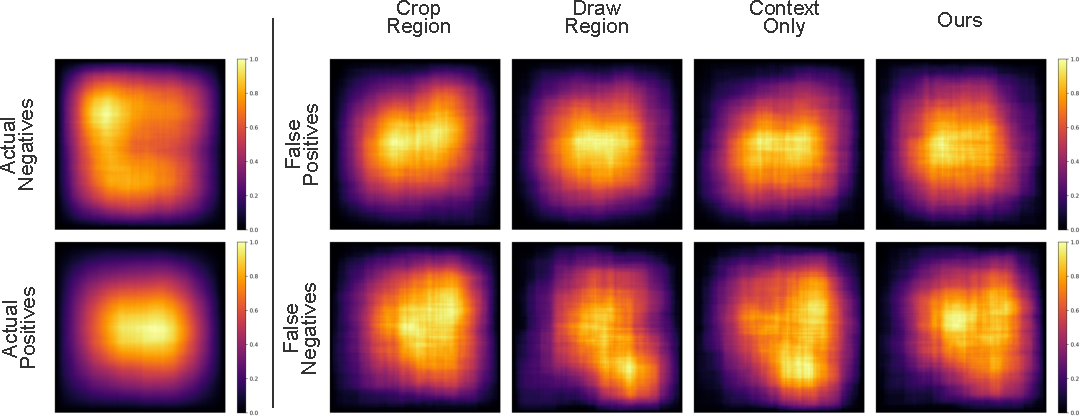
\includegraphics[width=\textwidth]{Figures/Part1_LocVQA/02_llm/supplementary_errors_by_location.pdf}
\caption{Error analysis by region location for the four strongest baselines for the RIS-VQA dataset. The maps are obtained by adding binary masks representing the regions for all QA pairs in each category and then normalizing.}
\label{fig:supplementary_errors_by_location}
\end{center}
\end{figure}

\begin{figure}[!h]
\begin{center}
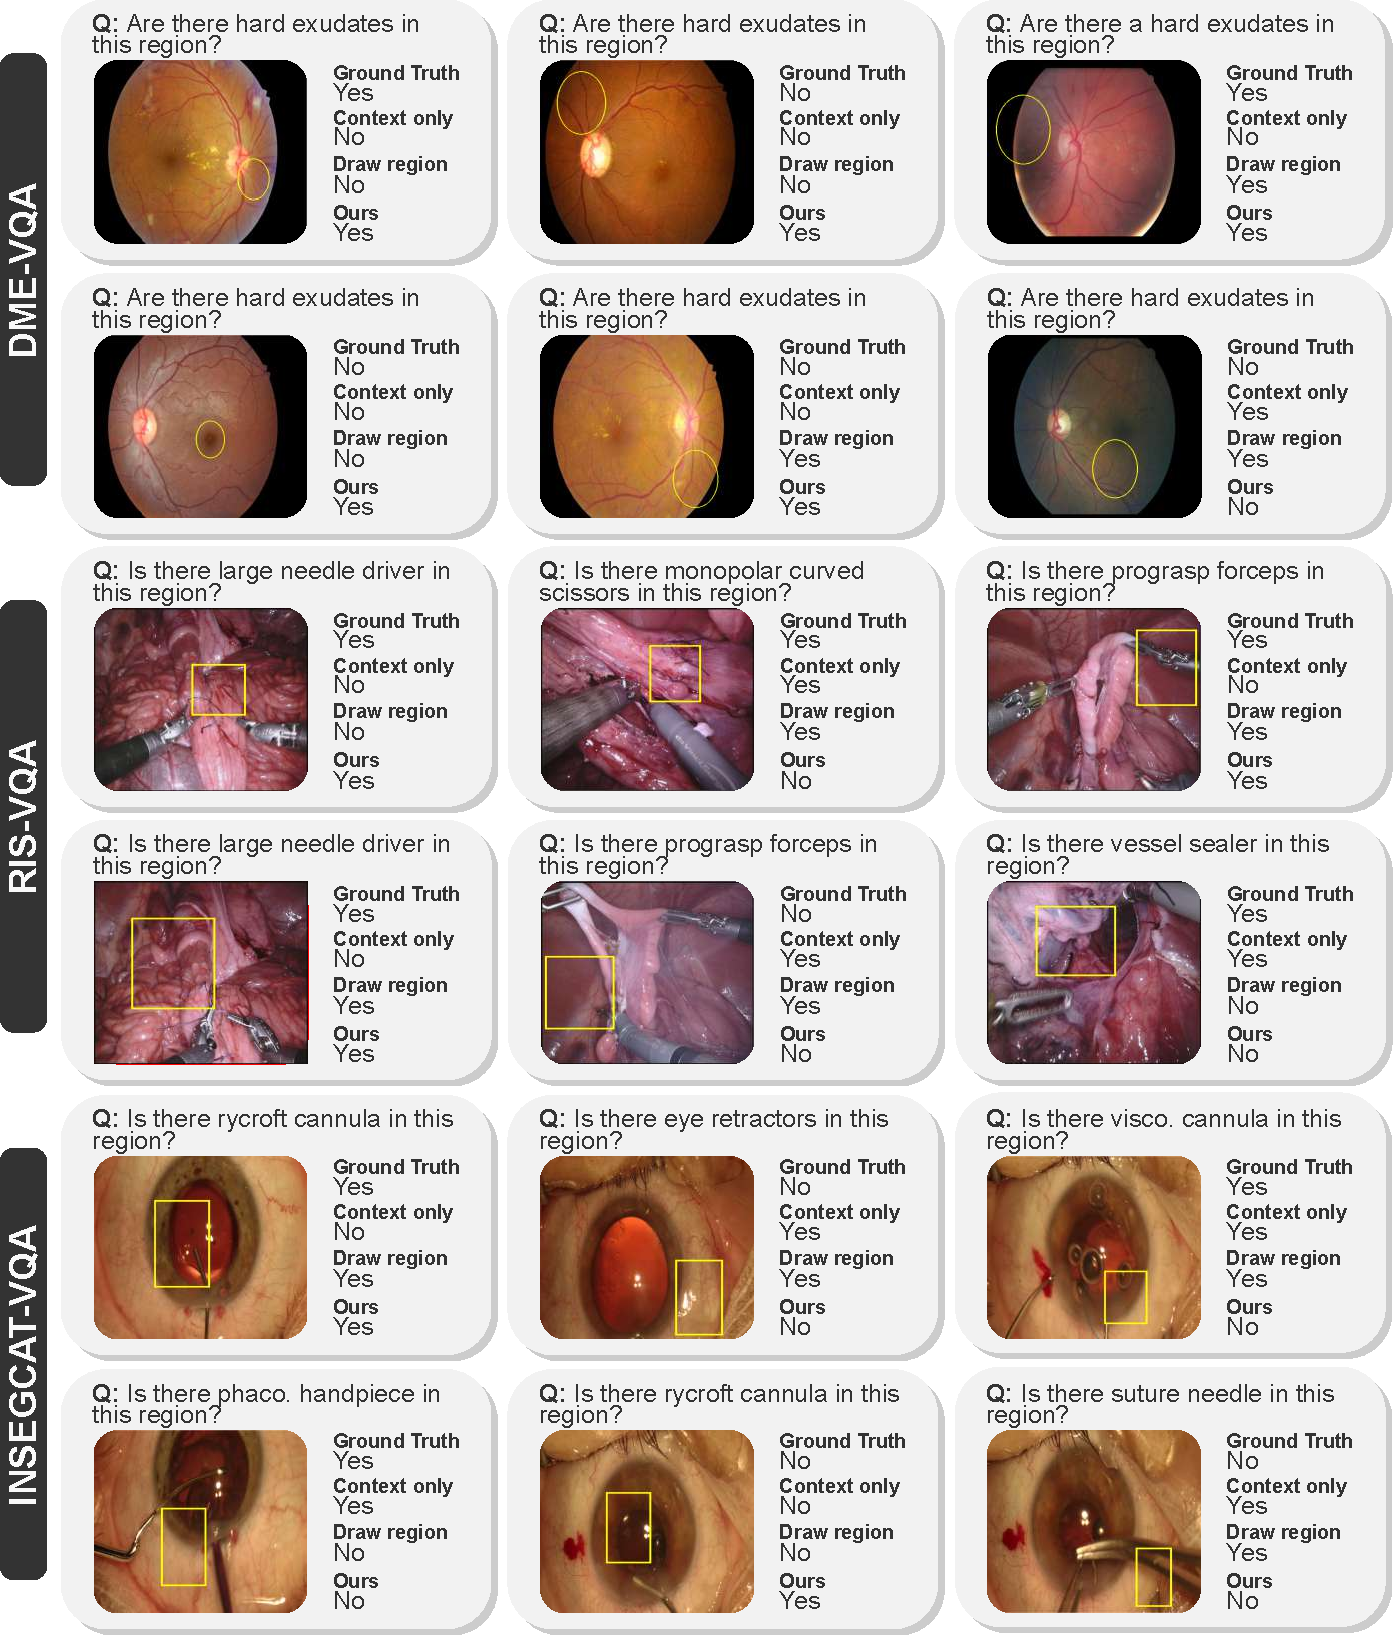
\includegraphics[width=\textwidth]{Figures/Part1_LocVQA/02_llm/examples_supplementary.pdf}
\caption{Additional examples for DME-VQA (rows 1 and 2), RIS-VQA (rows 3 and 4) and Insegcat-VQA (rows 5 and 6).}
\label{fig:examples_supplementary_dme}
\end{center}
\end{figure}